\section{Introduction}\label{sec:intro}
The Laplace transform, $ X(s) = \LT \lbrace x(t) \rbrace$, simplifies the analysis of complex networks by replacing network elements with their equivalent impedances.
Integro-differential operations in the time-domain become algebraic operations in the Laplace s-domain.

A first order network with an active element can be generalized by the model shown in Fig.~\ref{fig:first-order-network}.

\begin{figure}[htpb]
	\centering
	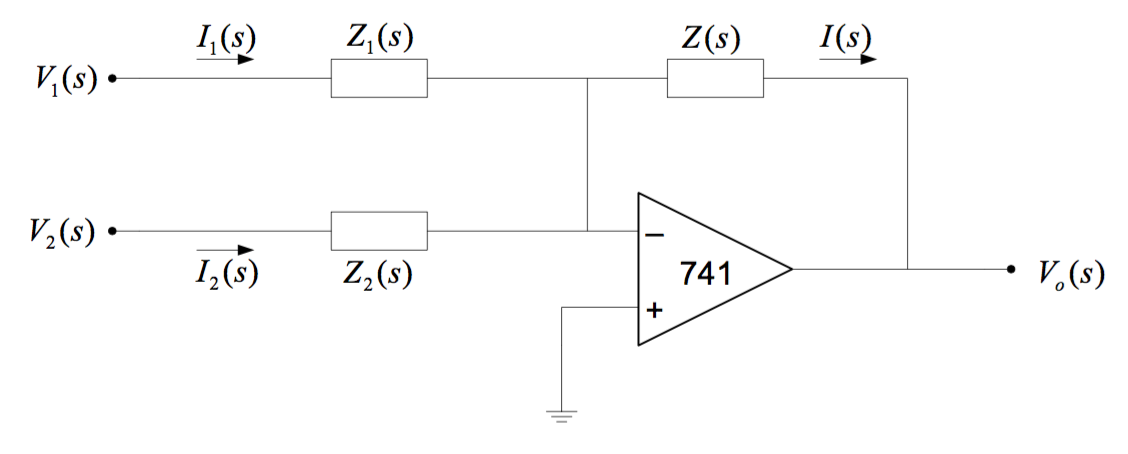
\includegraphics[width=0.7\linewidth]{graphics/s-network}	
	\caption{First order network in the s-domain}
	\label{fig:first-order-network}
\end{figure}

In the s-domain, the output is
\begin{equation}\label{eqn:first-order-network}
	V_o = - \left[ {Z \over Z_1}V_1 + {Z \over Z_2}V_2 \right]
\end{equation}
This general configuration gives rise to many different circuits depending on the values of $Z$, $Z_1$ and $Z_2$.

\paragraph{Inverting Voltage Amplifier} $Z = R$, $Z_1 = R_1$, $Z_2 = \infty$
\begin{equation}\label{eqn:inverter}
	V_o = - {R \over R_1}V_1
\end{equation}

\paragraph{Inverting Adder} $Z = R$, $Z_1 = R_1$, $Z_2 = R_2$
\begin{equation}\label{eqn:adder}
	V_o = - \left[ {R \over R_1}V_1 + {R \over R_2}V_2 \right]
\end{equation}

\paragraph{Inverting Integrator} $Z = {1 \over sC}$, $Z_1 = R_1$, $Z_2 = \infty$
\begin{equation}\label{eqn:integrator}
V_o = - {1 \over R_1 C} \cdot {1 \over s} V_1 = -G_1 {1 \over s} V_1
\end{equation}
In the time domain this becomes
\begin{equation*}
	v_o(t) = -G_1 \int_{0}^{t} v_1(\tau) d\tau.
\end{equation*}

\paragraph{Inverting Integrator} $Z = {1 \over sC}$, $Z_1 = R_1$, $Z_2 = R_2$
\begin{equation}\label{eqn:first-order}
V_o = - {1 \over s} \left[ {1 \over R_1 C} V_1 + {1 \over R_2 C} V_2 \right]
\end{equation}
